\documentclass[a4paper]{article}
\usepackage{graphicx}
\usepackage[utf8]{inputenc}
\usepackage{enumerate}
\usepackage{siunitx}
\sisetup{locale=DE} 
\usepackage{icomma}
\usepackage{amssymb}
\usepackage{tikz}
\usepackage{href-ul}
\hypersetup{
	colorlinks=true,
	linkcolor=blue,
	urlcolor=blue}
\usepackage{geometry}
\geometry{a4paper, top=15mm, left=15mm, right=15mm, bottom=15mm,
	headsep=10mm, footskip=12mm}

\begin{document}
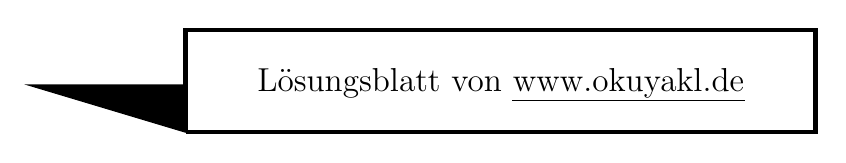
\begin{tikzpicture}(10,3)
	\draw[ultra thick](2,0) --(10,0) -- (10,1.3) --(2,1.3) -- (2,0);
	\draw[fill=black](2,0)-- (0,.6) -- (2,.6) -- (2,0);
	\node at (6,.6) {\large Lösungsblatt von \href{https://www.okuyakl.de}{www.okuyakl.de}};
\end{tikzpicture}
\vspace{0.5 cm}

\noindent {\bf Aufgabe 1. a)}\\
Die gesuchten Größen kann man mit der Formeln $P = U \cdot I$ und $U = R \cdot I$ berechnen:
$$
\renewcommand{\arraystretch}{2}
\begin{array}{rccl}
I_1 =& { P_1 \over U} =& {\SI{75}{\watt}\over \SI{230}{\volt} }=& \SI{0,33}{\ampere} \\
P_2 =& U \cdot I =& \SI{230}{\volt} \cdot  \SI{1,5}{\ampere} =&  \SI{345}{\watt} \\
I_3 =& {U \over R} =& {\SI{230}{\volt} \over  \SI{45}{\ohm} }=&  \SI{5,1}{\ampere} 
\end{array}
$$
\vspace{0.5 cm}

\noindent {\bf Aufgabe 1. b)}\\
Bei einer Parallelschaltung addieren wir die einzelnen Stromstärken. Dann ziehen wir sie von den $\SI{10}{\ampere}$ ab, die die Sicherung gerade noch durchlässt:
$$I_4 =  \SI{10}{\ampere} - (I_1+I_2+I_3)= \SI{10}{\ampere} -  \SI{0,33}{\ampere} -  \SI{1,5}{\ampere} -  \SI{5,1}{\ampere} =  \SI{3,1}{\ampere}$$
Das Gerät $G_4$ darf also maximal $\SI{3,1}{\ampere}$ durchlassen, dies entspricht einer Leistung von 
$$P= \SI{230}{\volt} \cdot  \SI{3,1}{\ampere} \approx  \SI{710}{\watt}.$$
\vspace{0.5 cm}

\noindent {\bf Aufgabe 2.}\\
,,Werden von {\it einem} Strom durchflossen" bedeutet, dass sie in Reihe geschaltet sind.
$$
\renewcommand{\arraystretch}{2}
\begin{array}{rccl}
R_1 =& {U_1 \over I} =& { \SI{9,0}{\volt} \over \SI{0,18}{\ampere}}=&  \SI{50}{\ohm} \\
U_2 =& R_2 \cdot I =&  \SI{150}{\ohm} \cdot  \SI{0,18}{\ampere} =& \SI{27}{\volt}\\
U_{ges}=& U_1 +U_2 =& \SI{27}{\volt} + \SI{9,0}{\volt}=& \SI{36}{\volt}
\end{array}
$$
\vspace{0.5 cm}

\noindent {\bf Aufgabe 3.}\\
Die Betriebsstromstärke von $I_B=\SI{0,4}{\ampere}$ darf nicht überschritten werden, wenn das Gerät an eine höhere Spannung angeschlossen wird. Der Gesamtwiderstand muss also mindestens sein:
$$R_{ges}={U \over I_B}=\SI{575}{\ohm}$$
Den Widerstand des Gerätes kann man aus den angegebenen Daten berechnen:
$$R_B = {\SI{110}{\volt} \over  \SI{0,4}{\ampere}}= \SI{275}{\ohm}$$
Für den in Reihe zu schaltende Vorwiderstand $R_V$ gilt:
$$R_{ges}= R_B + R_V \quad \Leftrightarrow \quad R_V= R_{ges}-R_B=\SI{300}{\ohm}$$
\vspace{0.5 cm}

\noindent {\bf Aufgabe 4. a)}\\
Der Widerstand $R_0$ eines Leiters mit der Länge $l$ und dem Querschnitt $A$ berechnet sich mit:
$$R_0= \varrho \cdot {l \over A}$$
Hierbei ist $\varrho$ der spezifische Widerstand, eine materialabhängige Konstante. Wenn die neue Länge $2l$ ist und der neue Querschnitt $3A$, dann ist der neue Widerstand $R_A:$
$$R_A= \varrho \cdot { 2 l \over 3 A} = \underbrace{\varrho \cdot { l\over A}}_{=R_0} \cdot {2 \over 3}=R_0 \cdot {2 \over 3}$$ 
\vspace{0.5 cm}

\noindent {\bf Aufgabe 4. b)}\\
Die Querschnittsfläche ist  $A=\pi r^2$. Wird der Radius $r$ verdoppelt auf $2r$, dann vervierfacht sich A zu $4A$ wegen $2^2=4$. Wenn nun auch die Länge vervierfacht wird, dann heben sich beide Effekte auf und der Widerstand verändert sich nicht:    
$$R_A= \varrho \cdot { 4l \over 4 A} =\varrho \cdot { l\over A}=R_0$$ 
\vspace{0.5 cm}

\noindent {\bf Aufgabe 5.}\\
Wir stellen die Formel für den spezifischen Widerstand nach der Querschnittsfläche $A$ um:
$$
\renewcommand{\arraystretch}{2}
\begin{array}{rccl}
R &=& \varrho \cdot {l \over A} &| \cdot A \\
A \cdot R &=& \varrho \cdot l   &| : R \\
A &=& \varrho \cdot {l \over R} & =\SI{0,017}{\ohm\cdot\milli\meter^2\over \meter}\cdot {2\cdot \SI{17,5}{\meter}\over \SI{0,2}{\ohm}}\\
A &=& \SI{3,0}{\milli\meter^2} & = \pi \cdot r^2 \\
r &=& \sqrt{A \over \pi} &= \sqrt{\SI{3,0}{\milli\meter^2}\over \pi}\\
r &=& \SI{1,0}{\milli\meter}
\end{array}
$$
\vspace{0.5 cm}

\noindent {\bf Aufgabe 6.}\\
Mit jedem weiteren parallel geschalteten Widerstand wird $R_{ges}$ kleiner und $I_{ges}$ größer.
\vspace{0.5 cm}

\noindent {\bf Aufgabe 7.} \\
Bei einer Parallelschaltung gilt:\\
(a) Der Gesamtwiderstand ist kleiner als jeder einzelne Widerstand:
 $$R_{ges}<R_1 \quad {\rm und} \quad R_{ges}<R_2$$
(b) Die größere Stromstärke gehört zum kleineren Widerstand und umgekehrt: 
$$I_1<I_2$$
(c) Es gibt nur eine Spannung: 
$$U_1=U_2$$
\vspace{0.5 cm}

\noindent {\bf Aufgabe 8. a)}\\
Für eine Reihenschaltung zweier Verbraucher muss die Betriebs\-stromstärke $I_B$ gleich sein.
Diese berechnen wir:
$$
\renewcommand{\arraystretch}{2}
\begin{array}{rcccl}
{\rm Lampe \quad 1:} \quad I_1 &=&  \SI{0,1}{\ampere}\\
{\rm Lampe \quad 2:} \quad I_2 &=& { \SI{1,2}{\watt} \over \SI{12}{\volt}} &=&  \SI{0,1}{\ampere}\\
{\rm Lampe \quad 3:} \quad I_3 &=& { \SI{4,0}{\volt} \over  \SI{20}{\ohm}} &=&  \SI{0,2}{\ampere}\\
\end{array}
$$
Beide Lampen leuchten optimal, wenn wir Lampe 1 und Lampe 2 auswählen. 
\vspace{0.5 cm}

\noindent {\bf Aufgabe 8. b)}\\
Die Betriebsstromstärke ist - wie oben erwähnt - $I_B=\SI{0,1}{\ampere}$, der Gesamtwiderstand ist 
die Summe der Einzelwiderstände, oder besser die Summe der Betriebs\-spannungen...
$$U_{ges}=\SI{4,0}{\volt} + \SI{12}{\volt} = \SI{16}{\volt}$$ 
...geteilt durch die Betriebsstromstärke:
$$R_{ges}={ U_{ges} \over I_B}={\SI{16}{\volt}\over \SI{0,1}{\ampere}}= \SI{160}{\ohm} $$
\vspace{0.5 cm}

\noindent {\bf Aufgabe 9.}\\
Bei einer Parallelschaltung addieren sich die Kehrwerte der Einzelwiderstände zum Kehrwert des Gesamtwiderstands:
$$
\renewcommand{\arraystretch}{2}
\begin{array}{rcl}
{1 \over R_{ges}} &=& {1 \over R_2} + {1 \over R_2}\\
R_{ges} &=& \left({1 \over R_2} + {1 \over R_2} \right)^{-1}\\
R_{ges} &=& \left({1 \over \SI{100}{\ohm}} + {1 \over \SI{300}{\ohm}} \right)^{-1}\\
R_{ges} &=& \SI{75}{\ohm}
\end{array}
$$
\vspace{0.5 cm}

\noindent {\bf Aufgabe 10.}\\
$$
\renewcommand{\arraystretch}{2}
\begin{array}{rccl}
U_2 =& U_{ges}=& R_2 \cdot I_2 =& \SI{36}{\volt} \\
I_1 =& {U \over R_1} =& { \SI{36}{\volt} \over \SI{4,0}{\ohm}}=& \SI{9,0}{\ampere} \\ 
I_3 =& {U \over R_3} =& { \SI{36}{\volt} \over \SI{24,0}{\ohm}}=& \SI{1,5}{\ampere} \\
I_{ges}=& I_1 +I_2+ I_3 =& \SI{4,5}{\ampere} + \SI{9,0}{\ampere} + \SI{1,5}{\ampere} =& \SI{15}{\ampere}\\
R_{ges}=& \left({1 \over \SI{4,0}{\ohm}} + {1 \over \SI{8,0}{\ohm}} + {1 \over \SI{24,0}{\ohm}}\right)^{-1}
=&  \SI{2,4}{\ohm} \\
\end{array}
$$
Alternativ kann man den Gesamtwiderstand auch mit der Gesamtstromstärke und der Spannung berechnen:
$$R_{ges}={U \over I_{ges}}={\SI{36}{\volt} \over \SI{15}{\ampere}}= \SI{2,4}{\ohm}$$
 
\begin{center}
	\includegraphics[width=7 cm]{../../viecher/endcomic.pdf}
	
	Hier geht es zurück zum \href{https://www.okuyakl.de/phys/p10elL101/aa101.pdf}{Aufgabenblatt}
\end{center}

\end{document}